\section{Künstliche Intelligenz}
\label{chap:KI}

Das Thema \ac{KI} hat in letzter Zeit durch den Chatbot ChatGPT der Firma OpenAI eine große mediale Aufmerksamkeit erhalten. 
ChatGPT wurde im November 2022 veröffentlicht und ist ein Sprachmodell, das natürliche Sprache verstehen und abhängig von der 
Benutzereingabe in Dialogform Antworten liefern soll. Es ist dabei in der Lage, sich an vorherige Eingaben zu erinnern und kann 
deshalb Anfragen in einen Kontext einordnen. Dadurch kann es auch vorherige Antworten korrigieren und auf Wünsche und Bedürfnisse 
des Benutzers eingehen \cite[]{CHATGPT}. 

Die Frage nach \ac{KI} und nach dem ob und wie Maschinen denken können ist jedoch wesentlich älter als dieser Chatbot. 
Bereits Alan Turing stellte sich diese Frage in den 1950er Jahren. Er schlug vor die Frage, ob Maschinen denken können,
mit einer anderen Frage zu ersetzen. Dafür formulierte er das Problem mithilfe eines Spiels, dem \glqq Imitation Game\grqq, 
das heute eher als Turing-Test bekannt ist, um. Dieses Spiel wird mit drei Personen gespielt, einem Fragesteller, einem Mann und 
einer Frau. Ziel des Spiels ist es, dass der Fragesteller mithilfe von Fragen herausfinden muss, welche Person der Mann und welche Person 
die Frau ist. Der Mann soll dabei versuchen, dass der Fragesteller ihn fälschlicherweise als die Frau identifiziert, während die Frau versuchen soll, 
dass der Fragesteller sie korrekt als Frau identifiziert. Dafür befindet sich der Fragesteller in einem anderen Raum und die Fragen werden entweder 
über eine außenstehende weitere Person oder einem Fernschreiber übermittelt. Was würde nun passieren, wenn eine Maschine die Rolle des Manns übernehmen würde?
Würde der Fragesteller dann häufiger oder seltener gewinnen \cite[vgl. S.433f.]{TURING}? Alan Turing glaubte, dass eine Maschine dann als
intelligent bezeichnet werden könne, wenn eine Maschine in der Lage dazu ist, menschliches Verhalten zu imitieren.

\begin{wrapfigure}[7]{r}{\textwidth/2}
    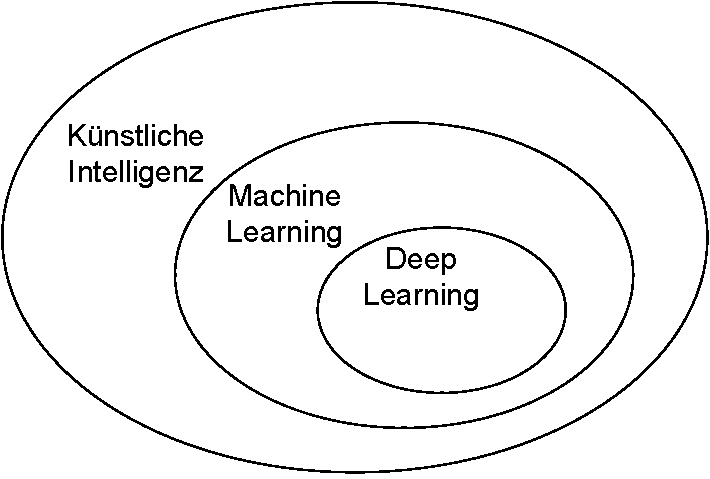
\includegraphics[width=\textwidth/2]{abbildungen/KI_ML_DL.pdf}
    \caption{Beziehung zwischen \ac{KI}, \ac{ML} und \ac{DL}}
    \label{fig:KI_ML_DL}

\end{wrapfigure} 

François Chollet, der Entwickler der Deep-Learning-Bibliothek Keras, welche im Kapitel XXX TODO näher beschrieben wird, definiert
das Fachgebiet \ac{KI} als \glqq [den] Versuch, normalerweise von Menschen erledigte geistige Aufgaben automatisiert zu lösen\grqq \cite[S.22]{DL_PY}.
Nach dieser Definition schließt \ac{KI} weitere Themen wie das Machine Learning sowie das Deep Learning ein. Wichtig zu beachten ist dabei,
dass diese Gebiete sich voneinander unterschieden. Ihre Beziehung zueinander wird in Abbildung \ref*{fig:KI_ML_DL} verdeutlicht.
%\begin{figure}[H]
%    \begin{minipage}[t]{\textwidth/2 - 1cm}
%        \vspace{0pt}
%        \centering
%        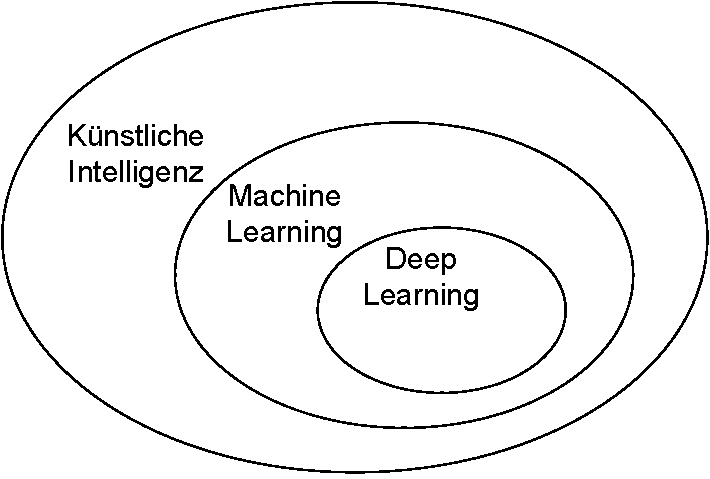
\includegraphics[width = \textwidth]{abbildungen/KI_ML_DL.pdf}
%        \caption{Beziehung zwischen \ac{KI}, \ac{ML} und \ac{DL}}
%        \label{fig:KI_ML_DL}
%    \end{minipage}
%    \hfill
%    \begin{minipage}[t]{\textwidth/2}
%        \vspace{0pt}
%        François Chollet, der Entwickler der Deep-Learning-Bibliothek Keras, welche im Kapitel XXX TODO näher beschrieben wird, definiert
%        das Fachgebiet \ac{KI} als \glqq [den] Versuch, normalerweise von Menschen erledigte geistige Aufgaben automatisiert zu lösen\grqq \cite[S.22]{DL_PY}.
%        Nach dieser Definition schließt \ac{KI} weitere Themen wie das Machine Learning sowie das Deep Learning ein. Wichtig zu beachten ist dabei,
%        dass diese Gebiete sich voneinander unterschieden. Ihre Beziehung zueinander wird in Abbildung \ref*{fig:KI_ML_DL} verdeutlicht.
%    \end{minipage}
%\end{figure}

%\begin{figure}[h]
%    \centering
%    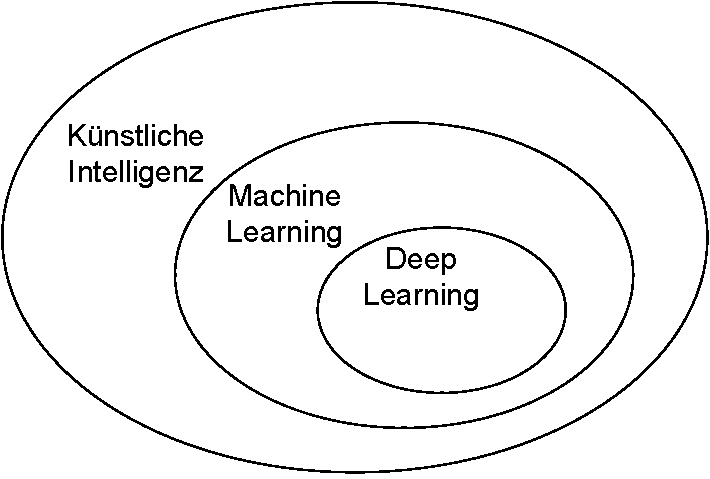
\includegraphics[]{abbildungen/KI_ML_DL.pdf}
%    \caption{Beziehung zwischen \ac{KI}, \ac{ML} und \ac{DL}}
%    \label{fig:KI_ML_DL}
%\end{figure}

\subsection{Maschinelles Lernen}



